%%==================================================
%% chapter05.tex for SJTU Master Thesis
%% based on CASthesis
%% modified by wei.jianwen@gmail.com
%% version: 0.3a
%% Encoding: UTF-8
%% last update: Dec 5th, 2010
%%==================================================

%\bibliographystyle{sjtu2} %[此处用于每章都生产参考文献]
\raggedbottom
\chapter{实验与分析}
\label{chap:evaluation}
%向下 或 向上 取整的小优化

% 1,单位长度的误差方差比对,3种  diffGen,已调整/未调整)。 设置高度,画5个图
% 横坐标 第i个叶子,纵坐标 标准差  x 4(4个高度,4,7,10,13)  1,1  0.5   递增,因为层数越高 代价越小 噪音越大
% 横坐标  高度,纵坐标平均每个叶子的标准差1,2

% 应该是 每个error(i),有new - baseline  与  noise - baseline。然后  sum[error(i)]

% 2,内部节点。一样 也是5个图
%\part{title} 横坐标 第i个节点,纵坐标 标准差  x 4(4个高度,4,7,10,13)2,1
% 横坐标  高度,纵坐标平均每个节点的标准差2,2



% 3, 范围查询 。首先还是单点,内部节点的单点。比对 已调整/未调整 的差别,此时不比叶节点了
% 然后是范围查询情况,扯扯淡 因为没法设计啊  好像能设计诶 。 通过 c45肯定可以说明
% 横坐标  范围从2,3,4.。。。。。。,纵坐标,对应的标准差   5个图   3


% 4,找个推荐算法

\section{引言}

在前面的章节中,我们指出面向分类应用的差分隐私算法在范围计数查询需求中存在的噪音线性叠加的问题。接着详细介绍基础算法DiffGen与优化方案$BoostH$,并分析二者间的联系,说明DiffGen算法的相关特性。然后从一致性约束出发,基于最小二乘法的目标式设计并实现优化算法DiffCon。通过新的应答查询模式和噪音分布调整公式,达到优化单位和范围查询中发布数据准确度的目的。最后从理论角度,由误差方差对优化性能做了讨论总结。

本章节为课题的实验部分,将在多个方面对DiffCon算法进行比对实验,通过真实数据集测试算法的准确度,验证第四章中关于噪音误差方差的理论性能分析情况,最后引入真实分类应用场景的性能测试实验。主要工作包括:实验数据集、平台介绍;实验方案的设计;实验结果的分析说明。

\section{实验平台及设置}

\subsection{实验平台介绍}

首先介绍实验的硬件环境:
\begin{enumerate}
	\item 处理器:Intel® Core™ i5-3470 @ 3.20GHz,拥有2个物理内核(Physical Core),利用Hyper-Threading技术实现4个逻辑内核(Logical Core)。
	\item 内存:16G,硬盘:500G
\end{enumerate}

软件环境为:
\begin{enumerate}
	\item 操作系统为Windows 7旗舰版
	\item 编码语言为C++,采用Microsoft Visual Studio Community 2013集成开发环境。
	\item 使用matplotlib绘图
\end{enumerate}

\subsection{数据集简介}

实验部分的所有测试均基于真实数据集Adult\footnote{\url{https://archive.ics.uci.edu/ml/datasets/Adult}}\cite{adult}。它共有48863个样本,由6个连续属性、8个离散属性构成,类属性是对收入水平的判断,有2个两属性值“$\leqslant$50$K$”和“$>$50$K$”。所有的属性及属性值显示如图\ref{fig:adult}:

\begin{figure}[!htp]
	\centering
	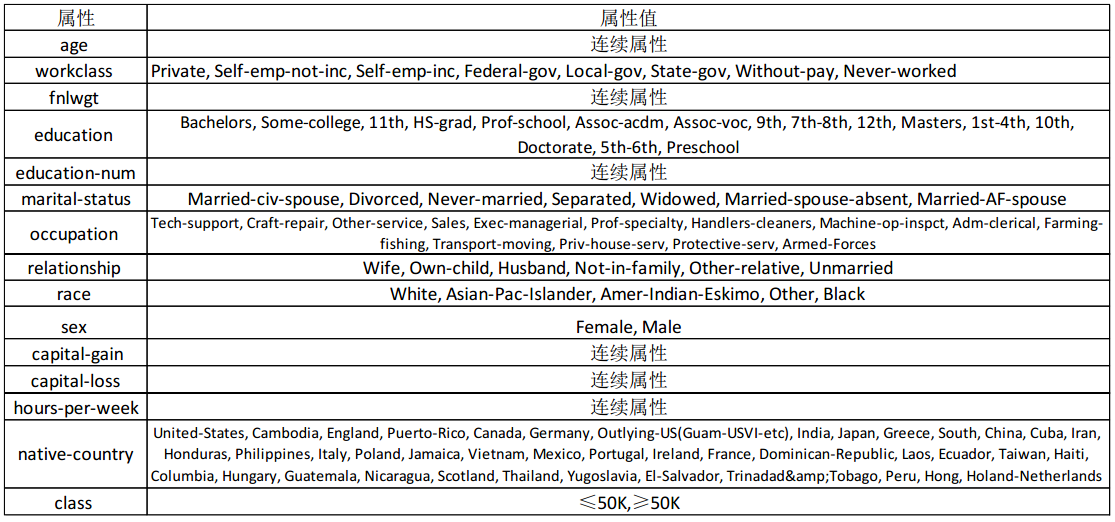
\includegraphics[width=5.8in]{chap5/adult}
	\bicaption[fig:adult]{图}{Adult数据集中的属性及属性值}{Fig.}{The attributes and attribte values in Adult dataset}
\end{figure}

由于在Adult数据集中存在着属性缺失的样本,因此在使用前需要进行处理。剔除不完整的样本之后,最终得到45222个可用的完整样本。

\section{实验设计概览}

本课题的目的是提升发布数据可用性,即提高数据在后续应用中的分类准确度,以此作为算法好坏的标准。因此,我们从理论测试和实践两个角度设计实验,概括如下:
\begin{enumerate}
	\item 验证理论分析结果。在\ref{theory analysis}节中,我们使用噪音的误差方差来评价算法的好与坏,作为衡量发布数据可用性的标杆。因此,在实验的第一部分中,我们比对三种不同应答查询模式下的误差方差:(1)往每个树节点加噪的初步方案$\tilde{L}_{all}(D)$。(2)基础算法DiffGen方式,即直方图模型$\mathcal{H}$,全局敏感性为1。(3)本课题的优化算法DiffCon方式$\tilde{\mathcal{H}}_{opt}$。在实验场景设计上,我们从单位长度查询和范围查询两个方面进行测试。方差能够使得两种数据的差距更加明显,但是,关注单一数据时,数据趋势的抖动会加剧,并且会导致实验图坐标的粒度太大,成倍淡化数值较小的数据分布特征。因此,采用标准差作为观察值。
	\item 真实分类算法上的实践。误差方差的理论测试难以替代真实场景的应用,因此通过C4.5分类器\cite{C45}来检测发布数据的分类准确度。同时,比对两个不同决策树分类算法的影响:IG(信息增益算法,Information Gain)和Max\cite{max}(最大值算法),最后分析实验结果。
	\item 对原数据集进行训练集与测试集的划分。针对分类应用的算法特性,将数据集按一定比例切分为训练集与测试集两个部分,接受完全相同的匿名化处理过程(参照\ref{chap4_class}节与DiffCon算法实现),最终生成两个新的发布数据集,作为分类应用测试的训练集和测试集输入。
\end{enumerate}	

\section{单位长度查询的测试与分析} 
\subsection{实验方案}
%跑几次,如何取平均
单位长度查询实验通过Adult数据集生成同一$DTree$树结构,比对3种应答查询模式下叶节点计数值的误差标准差。由于$DTree$可由树高控制,因此设定4种树高\{4,7,10,13\}场景,依次抽取20,50,100,200个叶节点,统计每个叶节点上类计数的误差标准差分布情况。对于每种树高情况,我们运行20次实验,取结果的平均值做结果分析。单位长度查询实验的关键代码如下:
\begin{lstlisting}[language={C++}, caption={单位长度查询实验}]
TestVariance_InEachLeafNode_Lall_DiffGen_DiffCon(){
	ofstream fout("TestVariance_InEachLeafNode_result.txt", ios::app);
	vector<HNode*> leaves = getleaves();   // 得到当前DTree树中的所有叶节点
	double Lall, diffgen, diffcon;  // 记录每个叶节点标准差的变量
	for (int i = 0; i < leaves.size(); i++){   
		Lall = diffgen = diffcon = 0;       
		for (int j = 0; j < getClassesNum(); ++j){  // getClassesNum()表示类属性个数,遍历每个类属性
			Lall += sqrt(pow((leaves[i]->noisy[j]), 2));   // noisy表示$\tilde{L}_{all}(D)$方式加的噪音
			diffgen += sqrt(pow((leaves[i]->DiffGenNoise[j]), 2));  //DiffGenNoise表示DiffGen方式加的噪音
			diffcon += sqrt(pow((leaves[i]->DiffConNoise[j]), 2));  //DiffConNoise表示DiffCon方式加的噪音
		}
		//取类属性计数值的平均误差标准差
		Lall = Lall / (double)(get_nClasses());  
		diffgen = diffgen / (double)(get_nClasses());
		diffcon = diffcon / (double)(get_nClasses());
		//写入第i个叶节点在三种查询应答模式下的误差标准差结果
		fout << Lall << " ";  
		fout << diffgen << " ";  
		fout << diffcon << endl; 
	}
	fout.close();
}
\end{lstlisting}
代码的注释对具体实验方案进行了完整解读,总体思路是计算每个叶节点在三种查询应答模式下的误差标准差结果,并写入结果文件中。在处理数据集的多个类属性情况时,我们统一取类属性计数值的标准差平均数作为计算结果,避免了为每个类属性维护统计分布的复杂情况。

在基于微观范围、关注于分布趋势的细粒度测试之后,接下来我们设计了粗粒度的整体实验,测试4种树高\{4,7,10,13\}场景下,每种查询应答模式下单位长度查询结果的平均误差方差情况,从宏观角度观察树高对误差方差的影响以及三种模式的性能优劣。具体实现上,统计每种模式下所有节点的误差方差总和,再除以节点数即可。

%平均单位长度的设计

\subsection{实验结果及分析}

三种查询应答模式与图例中的标记对应关系如表\ref{chap5_table1}所示。
单位长度查询的实验结果如图\ref{fig:EachLeaf},4个子图对应于树高Tree Height = 4,7,10,13,横坐标是枚举每个抽取到的叶节点,坐标值x表示$Dtree$的第x个叶节点,也就是第x个单位长度数据项;纵坐标是误差标准差的计算值,坐标值y越大,表示标准差越大,单位查询结果稳定性越差,也就是偏离真实结果的距离越大,准确度越低。

\begin{figure}[!htp]
	\centering
	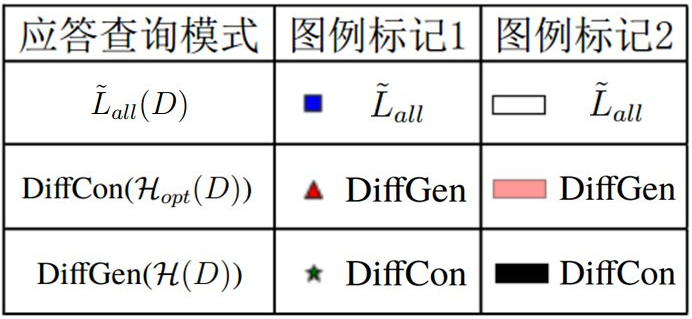
\includegraphics[width=3.5in]{chap5/RelationalTable}
	\bicaption[chap5_table1]{表}{查询应答模式与图例标记的对应关系表}{Table}{The relational table between inquiry-response mode and legend}
\end{figure}


\begin{figure}[!htp]
	\centering
	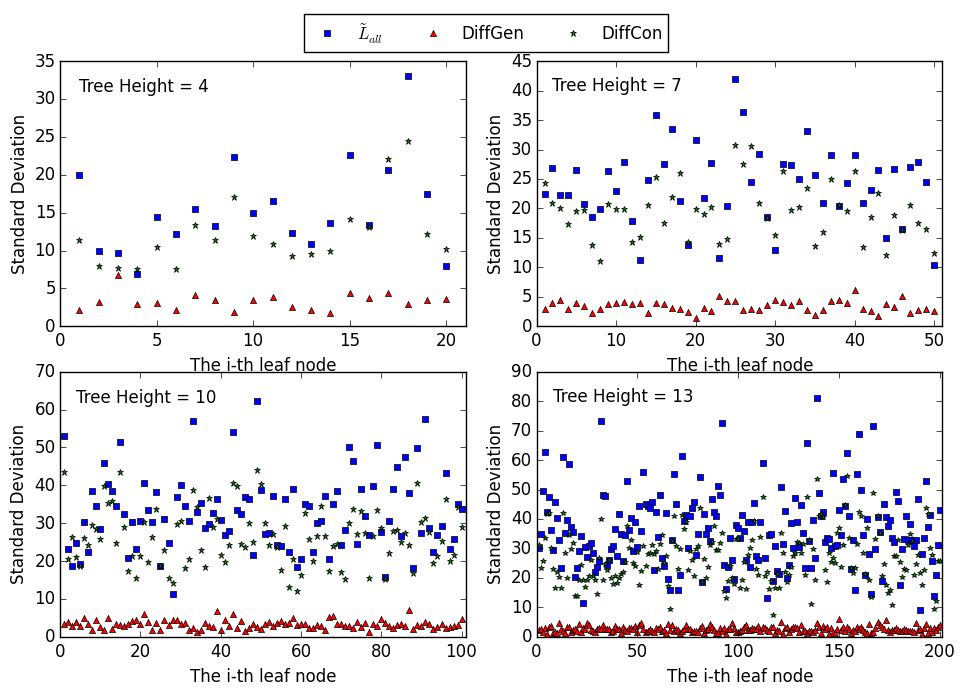
\includegraphics[width=6in]{chap5/EachLeaf}
	\bicaption[fig:EachLeaf]{图}{单位长度查询的实验结果}{Fig.}{The experimental result for unit-length queries}
\end{figure}

从实验结果来看,可观测到3个实验现象:(1)对于单位长度查询需求而言,DiffGen返回的应答结果距离真实值最近,并且分布相对稳定。(2)$\tilde{L}_{all}$和DiffCon都不是很稳定,在应答结果准确度上都劣于DiffGen,同时DiffCon优于$\tilde{L}_{all}$---对于同一X值,绝大部分的DiffCon点的Y值小于$\tilde{L}_{all}$的,树高4和7的实验结果比较容易看出。(3)随着树高的增加,误差标准差递增(如Y轴刻度值所示,在下个实验中更容易看出)。

导致DiffCon和$\tilde{L}_{all}$的误差标准差分布不稳定以及在应答准确度上均劣于DiffGen的原因,主要在于全局敏感性较大的缘故,都是树高$TH$。在差分隐私技术中,更大的全局敏感性决定了需要添加更多的噪音来保护隐私,在每个节点上所加噪音的量级为$Laplace(TH/\varepsilon)$,显然大于DiffGen的$Laplace(1/\varepsilon)$。因此更多的噪音扰动自然而然降低了应答准确度,同时,由于拉普拉斯概率密度函数是按照指数分布变动的布朗运动,更大的全局敏感性导致的是指数式的概率增减,加剧了函数结果的随机性,所以$\tilde{L}_{all}$和DiffCon不稳定。

单位长度查询的平均误差标准差实验结果如图\ref{fig:average_eachleaf},横坐标表示树高,纵坐标表示误差标准差的计算值。由实验结果观察到2个现象:(1)DiffGen返回的应答结果准确度最优,DiffCon次之,$\tilde{L}_{all}$最差。此现象的原因分析前文已论述过。(2)三种应答查询模式随着树高的增加,误差标准差随之增加(DiffGen起伏较小,但经多组实验观测也满足这个规律),产生这个现象的原因在于全局敏感性的定义上。随着树高的增加,由于$DTree$构建算法\ref{diffgen}中需要对隐私代价$\varepsilon$根据树高进行切分。显然,随着树高的增加,切分得越细,作为加噪参数分母部分的${\varepsilon}'$越小,噪音量级$Laplace(S(\mathcal{F})/{\varepsilon}')$越大,故此误差增加。

\begin{figure}[!htp]
	\centering
	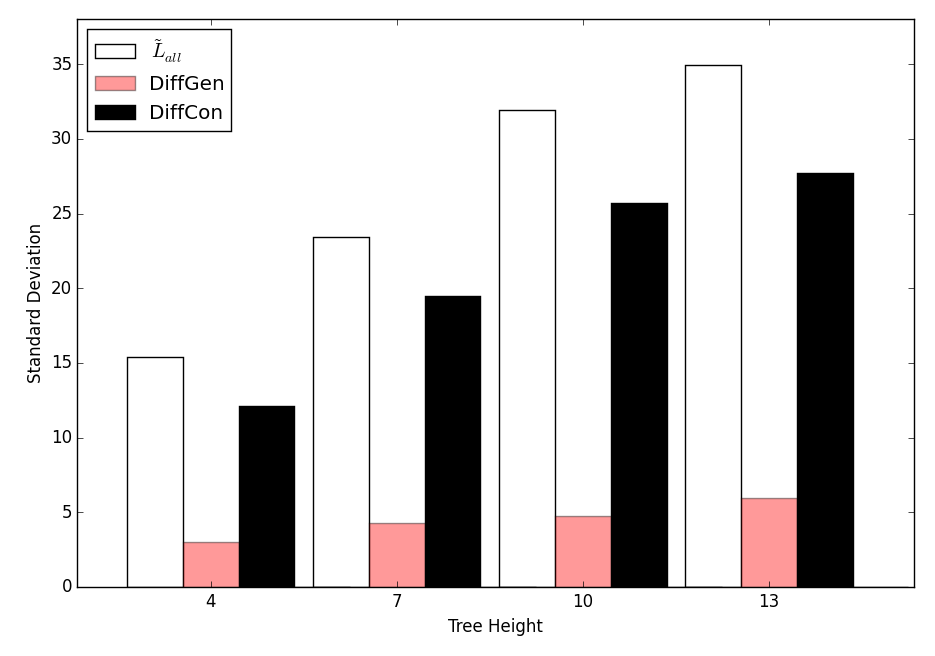
\includegraphics[width=5.3in]{chap5/average_eachleaf}
	\bicaption[fig:average_eachleaf]{图}{单位长度查询的平均误差标准差实验结果}{Fig.}{The mean standardized result for unit-length queries}
\end{figure}


\section{范围查询的测试与分析}
\subsection{实验方案}

范围查询实验的目的是分析不同应答查询模式对应答返回结果准确度的影响。根据前文的论述,理论上基于TMSC算法的DiffCon能够使用尽可能少的父节点来覆盖范围区间内的子节点,通过减少噪音线性叠加现象来取得优于DiffGen算法的效果。本着验证此理论假设的目的,我们按树高\{4,7,10,13\}根据不同的范围尺寸(即查询维度)设计了本节实验,查询范围的增加在实验中是通过取更多的叶节点来模拟。

我们通过Adult数据集生成同一$DTree$树结构,比对DiffGen和DiffCon算法在各种范围查询需求中返回应答的误差标准差情况,设定X轴自变量为范围尺寸,Y轴输出量为误差方差值。经过多次实验结果观察,两个算法的实验表现在较大X值时,其Y值处在不同量级水平,在同一散点图中Y值较小一方的实验规律几乎不可见;并且二者实验表现规律循环出现,因此取较小X值范围分析实验结果。我们取20,30,40,50的范围尺寸,对于每种范围尺寸运行20次实验,取结果的平均值做结果分析。范围查询实验的关键代码如下:
\begin{lstlisting}[language={C++}, caption={范围查询实验}]
TestVariance_RangeQuery_DiffGen_DiffCon(){
	ofstream fout("TestVariance_RangeQuery_DiffGen_DiffCon_result.txt", ios::app);
	......
	map<int, double> rangesize_variance_DiffGen; // DiffGen的map:rangesize->标准差总和
	map<int, double> rangesize_variance_DiffCon; // DiffGen的map:rangesize->标准差总和
	map<int, int> EachRangeNum;// map:rangesize->此rangesize中有多少个范围应答标准差相加
	vector<HNode*> leaves = getleaves();  //取叶节点
	int rangesize; //范围尺寸,从2开始,上限为覆盖所有叶节点
	for (rangesize = 2; rangesize <= leaves.size(); rangesize++){
		sumDiffGen = sumDiffCon = 0;
		for (int i = 0; i <= leaves.size() - rangesize; i += rangesize){
			rDiffGen = rDiffCon = 0; //初始化临时变量
			diffgen.resize(rangesize); diffgen.resize(rangesize);
			for (int j = i; j - i < rangesize; j++){
				for (int c = 0; c < get_nClasses(); ++c){
					diffgen[c] += sqrt(pow((leaves[j]->DiffGenNoise[c]), 2));
					diffcon[c] += leaves[j]->DiffConNoise[c];
					}	
			}
			for (int c = 0; c < getClassesNum(); ++c){
				diffcon[c] = sqrt(pow(diffcon[c], 2));
				rDiffGen += diffgen[c]; rDiffCon += diffcon[c];
			}
			// 取类属性分布的平均误差标准差
			rDiffGen = rDiffGen / (double)(getClassesNum());
			rDiffCon = rDiffCon / (double)(getClassesNum());
			sumDiffGen += rDiffGen;	sumDiffCon += rDiffCon;
			EachRangeNum[rangesize]++;
		}
		// 记录此rangesize下所有应答标准差的总和
		rangesize_variance_DiffGen[rangesize] = sumDiffGen;
		rangesize_variance_DiffCon[rangesize] = sumDiffCon;
	}
	for (int rangesize = 2; rangesize <= leaves.size(); rangesize++){
		// 此rangesize的平均应答标准差 = 标准差总和 / 范围应答个数
		rDiffGen = rangesize_variance_DiffGen[rangesize] / EachRangeNum[rangesize];
		rDiffCon = rangesize_variance_DiffCon[rangesize] / EachRangeNum[rangesize];
		fout << rangesize << " " << rDiffGen << " " << rDiffCon << endl; // 写入文件
	}
	fout.close();
}
\end{lstlisting}
代码的注释对具体实验方案进行了解析,总体思路是计算每种范围尺寸的平均应答标准差,通过HashMap维护每种范围尺寸与相关标准差的映射关系。需要注意的是,DiffGen与DiffCon标准差计算方式上的差异,参照代码14-25行。DiffGen的应答方式属于一维直方图方式,直接累加查询范围内的叶节点,因此每个叶节点的标准差单独计算。而DiffCon可利用一致性特性,尽可能地通过叶节点叠加得到最小的父节点覆盖集(TMSC算法思想),然后计算父节点集合的标准差。处理数据集的多个类属性情况依旧取类属性计数值的平均标准差作为计算结果。


\subsection{实验结果及分析}


由于DiffGen和DiffCon在Y值上的表现差距太大,过大的Y轴刻度间隔能满足DiffGen的分布需要,但是模糊了DiffCon散点的分布趋势,基本呈现为一直线。因此,对于每个子图,采用放大DiffCon散点分布的方法补充放大图。实验结果如图\ref{fig:figure_1}、\ref{fig:figure_2}、\ref{fig:figure_3}、\ref{fig:figure_4},根据箭头所示,每个子图右边是DiffCon分布趋势的放大图。4个子图分别对应于树高Tree Height = 4,7,10,13,横坐标是范围尺寸,纵坐标是误差标准差的计算值,坐标值y越大,表示结果稳定性越差,准确度越低。

\begin{figure}[!htp]
	\centering
	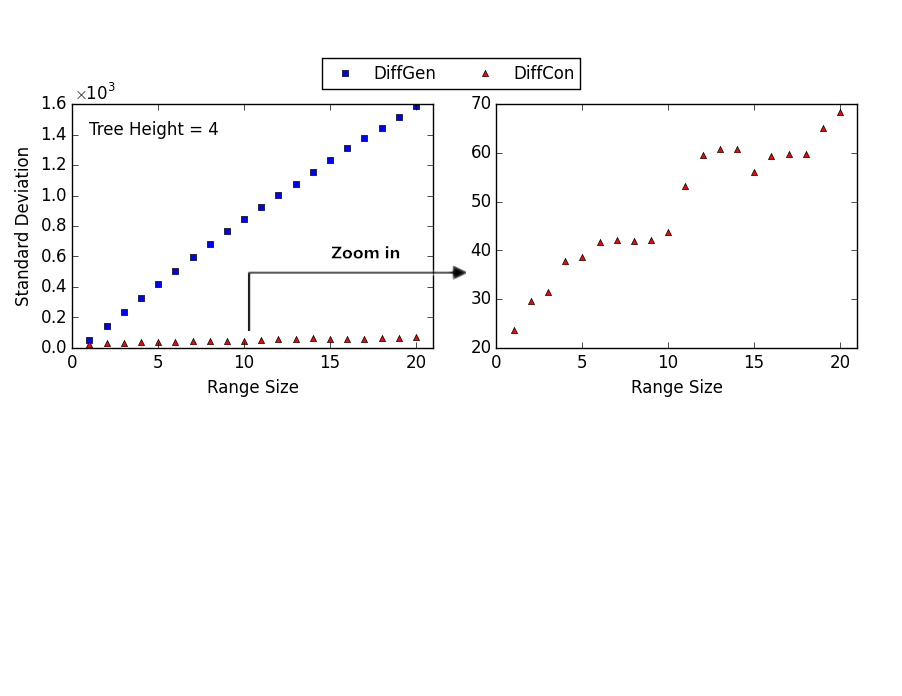
\includegraphics[width=5.5in]{chap5/figure_1}
	\bicaption[fig:figure_1]{图}{树高为4时的范围查询实验结果}{Fig.}{The experimental result of range query when Tree Height is 4}
\end{figure}

\begin{figure}[!htp]
	\centering
	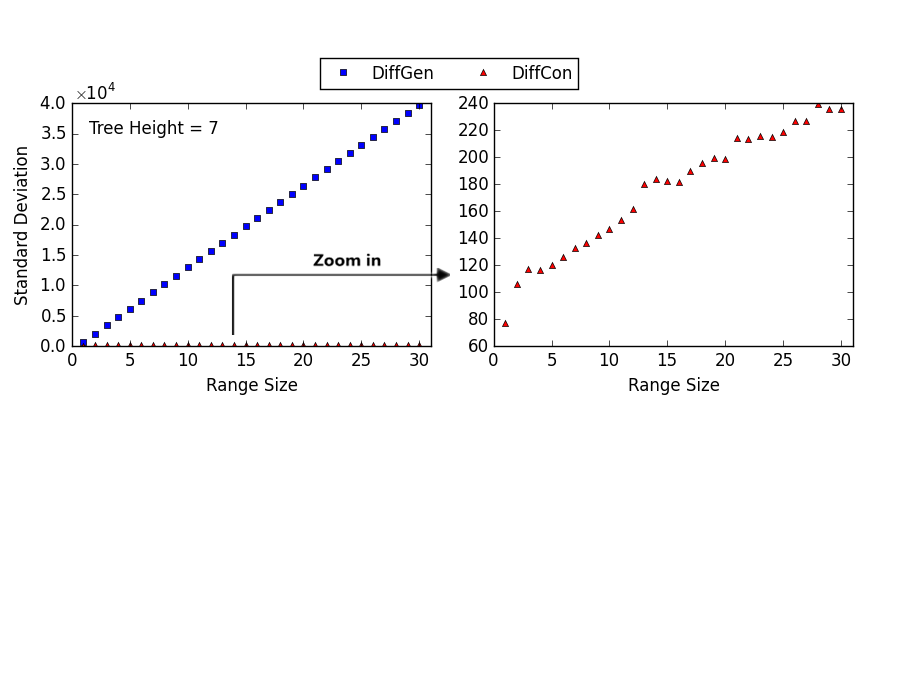
\includegraphics[width=5.5in]{chap5/figure_2}
	\bicaption[fig:figure_2]{图}{树高为7时的范围查询实验结果}{Fig.}{The experimental result of range query when Tree Height is 7}
\end{figure}

\begin{figure}[!htp]
	\centering
	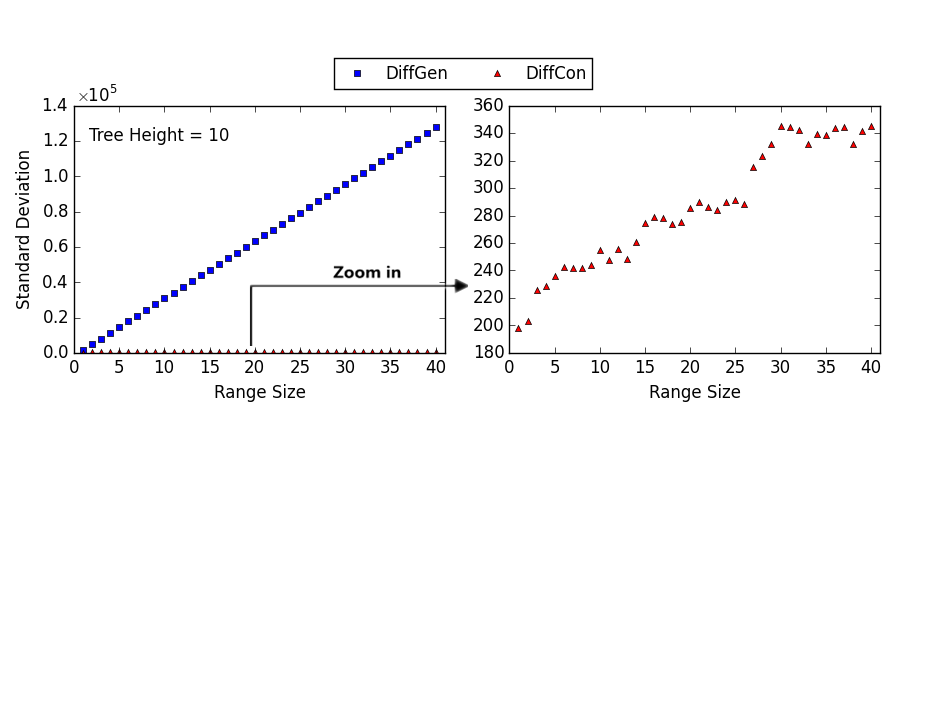
\includegraphics[width=5.5in]{chap5/figure_3}
	\bicaption[fig:figure_3]{图}{树高为10时的范围查询实验结果}{Fig.}{The experimental result of range query when Tree Height is 10}
\end{figure}

\begin{figure}[!htp]
	\centering
	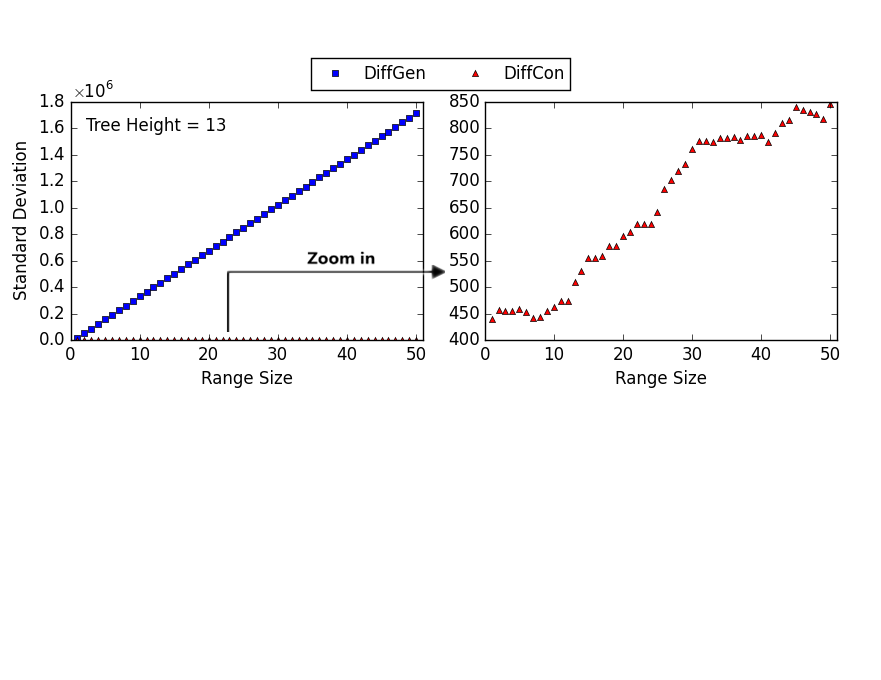
\includegraphics[width=5.5in]{chap5/figure_4}
	\bicaption[fig:figure_4]{图}{树高为13时的范围查询实验结果}{Fig.}{The experimental result of range query when Tree Height is 13}
\end{figure}

从实验结果来看,可观测到3个有意义的实验现象:
\begin{enumerate}
	\item[(1)]从左图的整体角度来看,随着X值的增加,DiffGen的误差标准差基本呈现线性的递增规律,DiffCon的误差标准差几乎为一常量。
	\item[(2)]通过右图的微观角度观察,随着X值的增加DiffCon散点趋势保持着缓慢的递增规律,并且在较多的X值区间中其标准差为定值,停止递增;在某些范围尺寸上Y值减小。
	\item[(3)]随着树高的增加,同一范围尺寸或整体的误差标准差情况(Y轴数值)均是呈现递增规律。
\end{enumerate}

基于这些实验现象,分别做研究分析:
\begin{enumerate}
	\item[(1)]根据前文的讨论,DiffGen的频率矩阵加噪模型本质使得它存在着噪音的线性叠加问题,在此实验现象中形象地体现了这一推论。在单位长度查询实验中由于仅仅涉及单个节点,敏感性的定义决定了它在单节点上有较好的噪音量级,因此优于DiffCon。但是基于单位长度数据项的查询应答模式决定了DiffGen在范围查询需求中的劣势,并且随着查询维度的增加,越发突出,印证了第二、第三章节的理论研究。
	\item[(2.1)]DiffCon的缓慢递增规律是由查询范围的增加所决定的必然结果。设想极端情况就很容易理解这一实验现象---比对最大范围查询(根节点)和单位长度查询(单个叶节点)的误差标准差。查询的范围越大,哪怕能不断找到覆盖查询范围的父节点(TMSC算法),最终的误差标准差趋势总是增加的。
	\item[(2.2)]在某些范围尺寸区间中,DiffCon的标准差表现为一恒定值,这是TMSC算法思想所产生的结果。查询范围的增加在实验中是通过取更多的叶节点来模拟,当新取到的叶节点$cur$与应答结果集合$\Upsilon$中的任何节点都不属于同一父节点,那么只能有
	\[
	\Upsilon \leftarrow \Upsilon + cur
	\]
	此时误差标准差增加。
	当$cur$正好与$\Upsilon$中的某节点集合$Set$属于同一父节点$parent$时,那么可用此父节点来覆盖$cur$与$Set$。这个过程为
	\[
	\Upsilon \leftarrow \Upsilon - Set - cur + parent
	\]
	也就是TMSC算法思想。那么,$Set$内的节点数|$Set$|成了DiffCon散点趋势恒定还是递减的关键。权衡在误差标准差上的两种损益情况:(a)剔除$Set$与$cur$得到的标准差获益。(b)增加$parent$产生的标准差损失。当二者相持平时,DiffCon散点趋势保持水平;当获益大于损失时,获得更好的误差标准差表现。
	\item[(3)]这个现象在单位长度查询实验中已经讨论过了,都是由于树高的增加导致隐私代价$\varepsilon$被切分地越细,加了更多的拉普拉斯噪音。
\end{enumerate}

\section{面向分类算法的测试与分析}

单位长度查询和范围查询是理论验证类型的实验,在现实使用中通过实践来验证算法的优劣将更具说服力。本节实验使用C4.5分类器,测试经过差分隐私匿名算法处理的发布数据集(Released dataset)在真实分类应用场景中的可用性。

\subsection{实验方案}

我们基于控制变量法设计DiffCon和DiffGen的比对实验,使用Adult数据集生成同一$DTree$树结构,从45222个样本中取30162个样本作为训练样本集,其余的用作测试样本集,并且保证训练/测试样本集在两个算法的运行过程中接受相同的的匿名化处理,两算法使用同样的训练/测试样本集。
由于$DTree$的构建算法影响着实验结果,因此针对两个不同的决策树算法---IG(信息增益算法)和Max(最大化算法),设计两组实验。在每组实验中,取4种隐私代价$\varepsilon$=0.1,0.25,0.5,1情况,分别测试不同树高对算法准确度的影响,X轴根据树高4,7,10,13,16设置5个值,Y轴为分类准确度(\%)。对于每个隐私代价值运行20次实验,取结果的平均值做为结果。

\subsubsection{方案流程及C4.5分类器的使用}

整体实验方案流程如图\ref{fig:c45process}。对于生成的发布数据集,可通过命令行的形式调用C4.5分类器$\footnote{\url{http://www2.cs.uregina.ca/~dbd/cs831/notes/ml/dtrees/c4.5/tutorial.html}}$测试数据集的分类准确度,指定输出文件参数即可得到结果,说明及示例图\ref{fig:c45cmd}所示。通过adult数据集生成了发布数据集ReleasedDataset,按照C4.5分类器语法指定参数,在最后的日志文件C4.5\_log.out中获取测试结果。

\begin{figure}[!htp]
	\centering
	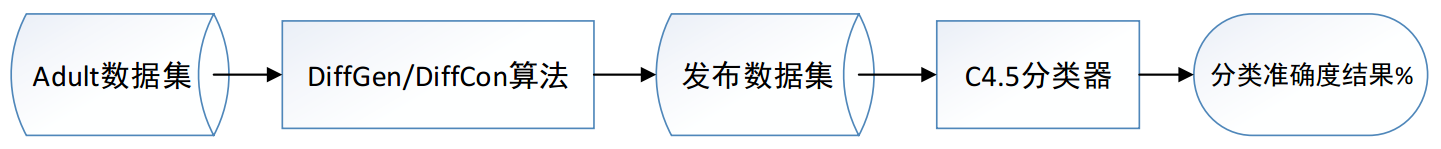
\includegraphics[width=5.5in]{chap5/c45process}
	\bicaption[fig:c45process]{图}{面向分类算法的实验流程}{Fig.}{The experimental procedure of algorithm based classification}
\end{figure}

\begin{figure}[!htp]
	\centering
	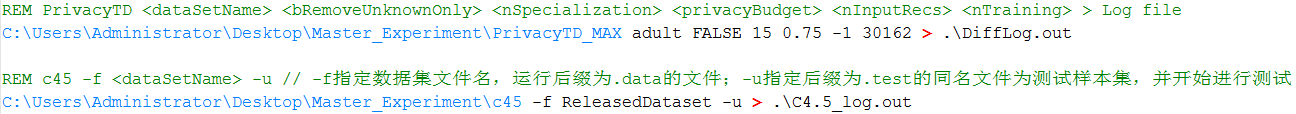
\includegraphics[width=5.5in]{chap5/c45cmd}
	\bicaption[fig:c45cmd]{图}{面向分类算法的实验流程}{Fig.}{The experimental procedure of algorithm based classification}
\end{figure}

\subsubsection{基准线}

借鉴DiffGen论文中的基准线设计,本实验设置了两个基准线Baseline与LowerBound,目的在于研究引入噪音的影响。Baseline完全使用原始数据集,不使用任何匿名化技术的测试结果,即未引入噪音且完全不保护隐私的测试场景,它可以用来衡量保护隐私而产生的准确度损失程度。LowerBound是仅仅保留类属性,移除其他所有属性的测试结果,即提供最大化的隐私保护力度,它可以用来衡量DiffGen/DiffCon算法取得的准确度收益。

设置了这两个基准线,就可以通过实验准确度与Baseline/LowerBound的差值衡量隐私保护力度和准确度之间的损益关系。因此,实验前先对Adult数据集做处理,运行C4.5分类器得到Baseline与LowerBound的准确度;然后根据不同的打分函数IG和Max,分组进行实验;最后统计实验结果。

\subsection{实验结果及分析}    

实验结果如图\ref{fig:ig}、\ref{fig:max},分别对应于IG和Max算法,Y轴表示20次重复计算的平均准确度,显然Y值越高算法性能越好。从实验结果图中主要呈现了3个实验现象,接下来分别进行分析探究。

\begin{figure}[!htp]
	\centering
	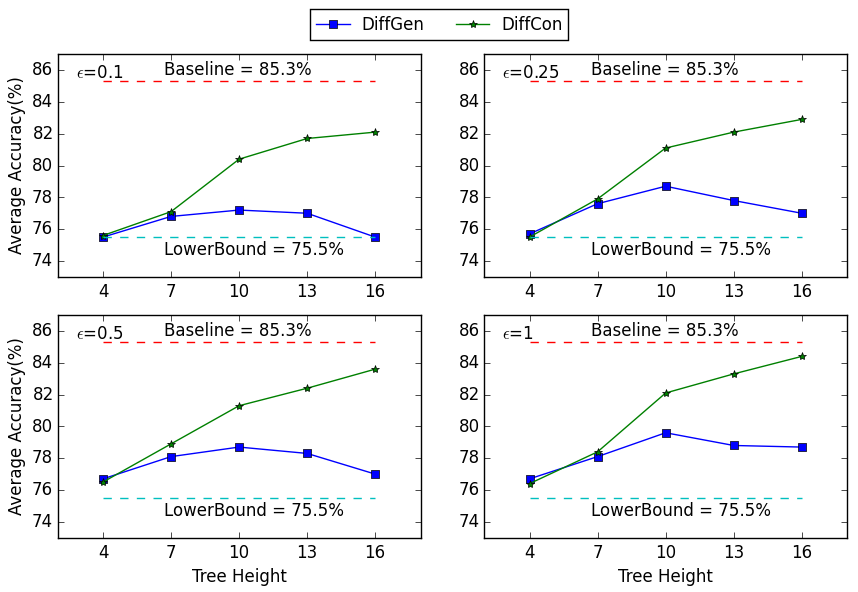
\includegraphics[width=5.5in]{chap5/IG}
	\bicaption[fig:ig]{图}{采用信息增益算法的分类准确度}{Fig.}{Classification accuracy in Information Gain}
\end{figure}

\begin{figure}[!htp]
	\centering
	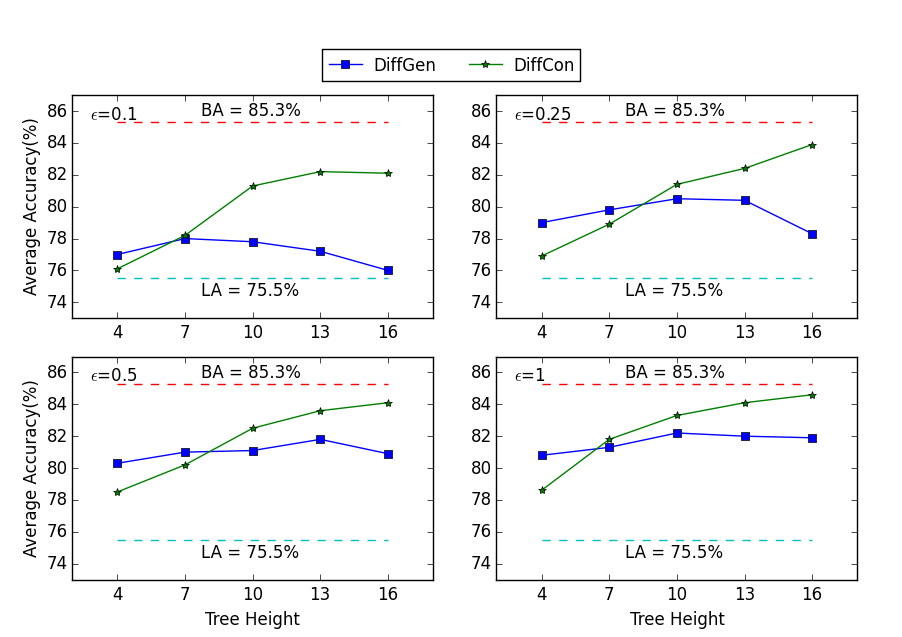
\includegraphics[width=5.5in]{chap5/MAX}
	\bicaption[fig:max]{图}{采用最大化算法的分类准确度}{Fig.}{Classification accuracy in Max}
\end{figure}

首先,整体情况上来看采用IG算法的实验效果不如Max算法。在$DTree$构建过程中采用指数机制选择分裂属性,而分裂属性选择得当与否决定了发布数据集的分类准确度。因此,Max算法对于DiffGen/DiffCon来说是个更“好”的打分函数,更适合于Adult数据集,在挑选分裂属性时偏向选出更有利于分类结果的属性。并且,Baseline的准确度最高,LowerBound最低,这个现象与设计原理相符。

其次,对于某个横坐标点产生的Y值,|Y-Baseline|与|Y-LowerBound|分别表示采用差分隐私技术、引入隐私代价$\varepsilon$后的准确度损失和收益。观测DiffGen曲线中同一X轴点对应的Y值,可以看到随着$\varepsilon$值的增加,|Y-LowerBound|逐渐变大,特别是在Max的实验结果图中,好像曲线在逐渐抬高。例如,图\ref{fig:max}中当树高取值为10,$\varepsilon$=0.1,0.25,0.5,1时,|Y-LowerBound|分别为1.7\%,5.2\%,5.6\%,6.7\%,表明准确度收益在不断增加。特别是当$\varepsilon$从0.1翻倍为0.25时,收益涨为原先的3倍。这是因为随着$\varepsilon$值的增加,隐私保护力度不断减弱,更少的噪音引入使得准确度收益呈现递增态势;换个角度来看,隐私保护带来的准确度损失的增长度劣于收益增长度。

这个现象对于DiffCon来说比较适合于树高为4和7的情况,随着$\varepsilon$值的增加,准确度收益|Y-LowerBound|递增,但是当树高超过7之后,这个现象变得不那么明显了。此时准确度收益递增缓慢是因为在当前树高情况下,准确度收益已经接近饱和状态。在DiffGen的曲线中,|Y-Baseline|与|Y-LowerBound|的差异不大,甚至在$\varepsilon$=0.1时以及IG实验结果中,前者更占上风,因此准确度收益与损失的差值既是提升的额度。DffGen极大化地利用$\varepsilon$的增加所带来的提升空间,因此准确度收益能不断递增。但是在DiffCon中,随着树高的增加,树节点呈指数式递增,$DTree$变得“枝繁叶茂”,此时它的范围查询优势就凸显了出来。所以,哪怕降低隐私保护需求带来了准确度提升空间,但DiffCon已经把准确度收益提升到了极致,|Y-LowerBound|超过|Y-Baseline|很多,已呈饱和状态。

最后,观察每个子图中DiffGen/DiffCon曲线的趋势。可以看到,DiffGen呈现先增加后下降的趋势,那是因为树高阈值对其产生的影响,比如树高为10。当树高小于某个阈值时,随着树高的增加$DTree$越显得“枝繁叶茂”,因此对于数据集中的每个属性来说,它越有可能被选中并按照匿名树结构进行分裂,在树节点中得到愈加“精确”的属性值呈现。例如,树高为1的仅由根节点组成的$DTree$,其数据集的类属性分布为布尔(Bool)分布,那么它的分类准确度最多为50\%;对它进行一次分裂生成2个子节点,理想情况下最高分类准确度能达到75\%。当树高大于某个阈值时,过多的树节点导致平均每个叶节点上的计数值被均摊地很小,甚至出现大部分为0的情况,因此发布出的数据集变得稀疏\cite{sparse_data_summary}。此时,加噪后的返回结果中,噪音总量占据了主要部分,发布数据集可用性大大降低。

DiffCon的曲线趋势是几乎为线性递增的趋势,受树高的影响很小。在DiffGen的树高阈值之前,DiffCon与DiffGen曲线差别不大,如树高为7。这是由于较小的$DTree$树高导致属性值分裂力度较弱,大部分属性在树节点中呈现较“模糊”的属性值,即属性值更靠近匿名树的根节点,有更大的泛化域。此时对于不同的“精确”的测试样本来说,很容易被归入同一树节点而得到一样的分类结果。因此,较小的树高使得不同属性值的区分边界变得模糊,DiffCon与DiffGen曲线差别很小。
当树高超过之前讨论的阈值时,DiffCon曲线依旧随着树高的增加而递增,如树高为10之后。与DiffGen一样,随着树高的增加落在叶节点上的待发布数据集也遇到了类计数值稀疏的问题,但是基于TMSC算法思想的应答查询模式和利用一致性特性的噪音调整算法,在解决此问题上收到了良好的效果。首先,DiffCon的噪音分布调整算法,能够使得$DTree$上的噪音分布更加平衡合理,对于类计数值较稀疏的叶节点来说,会分配到更少的噪音。其次,DiffCon的噪音量级是与查询范围的覆盖节点集合大小呈正比,不与叶节点数量线性相关,因此在叶节点的类计数值稀疏问题中,总能找到覆盖查询范围的较“稠密”的父节点集合,此时噪音总量不再占主导地位。最后,根据上节讨论随着树高的增加,隐私代价$\varepsilon$被划分的越细,会导致分类准确度损失|Y-Baseline|增加,但是此时的准确度收益|Y-LowerBound|的增长速率远远超过了损失速率。“枝繁叶茂”的$DTree$使得绝大部分的测试样本都能找到最“精确”的节点匹配,最大限度地发掘发布数据集的分类能力。

\section{本章小结}

